\chapter{Introduction}
\label{ch:intro}
\pagenumbering{arabic}

The intensive use of computational systems in the everyday of modern life creates the need for easier and less invasive forms of user recognition. While provide a correct password and place an expert to identify a person are the status quo respectively for verification and identification, voice biometrics presents itself as an alternative of continuous improvement. Passwords can be forgotten and people are biased and unable to be massive trained, but the unique characteristics of a person's voice combined with an Automatic Speaker Recognition (ASR) system outperform any ``manual" attempt.

Speech is the most natural way humans communicate, being incredibly complex and with numerous specific details related to its producer, \refbib{Bimbot et al.}{bimbot.et.al.2004}. Therefore, it is expected an increasing use of vocal interfaces to perform actions such as computer login, voice search (e.g., Apple Siri, Google Now and Samsung S Voice) and identification of speakers in a conversation and its content. Nowadays, fingerprint biometrics is present in several solutions (e.g., ATMs, \refbib{Wang \& Wu}{wang.wu.2002}), authentication through facial recognition comes as built-in software for average computers and iris scan was adopted for a short time by United Kingdom's and permanently by United Arab Emirates' border controls, \refbib{Sasse}{sasse.2007}, \refbib{Raisi \& Khouri}{raisi.khouri.2008}. These examples indicate a near future where biometrics is common, with people speaking with computers and cash withdrawals allowed through voice authentication.

Current commercial products based on voice technology (e.g., Dragon Naturally Speaking, KIVOX and VeriSpeak) usually intend to perform either \textbf{speech recognition} (\emph{what} is being said) or \textbf{speaker recognition} (\emph{who} is speaking). Voice search applications are designed to determine the content of a speech, while computer login and telephone fraud prevention supplement a memorized personal identification code with speaker verification, \refbib{Reynolds}{reynolds.1995a}. Few applications perform both processes, such as automatic speaker labeling of recorded meetings, that transcribes what each person is saying. To achieve these goals, several voice processing techniques have become known in academy and industry, such as Natural Language Processing (NLP), Hidden Markov Models (HMMs) and Gaussian Mixture Models (GMMs). Although all of these are interesting state-of-the-art techniques, this project covers a subarea of speaker recognition and only a small subset will be unraveled.

\section{Speaker Recognition}
\label{sec:speaker-recognition}

As stated in \refbib{Reynolds \& Campbell}{reynolds.campbell.2008}, speaker recognition is divided in two major subareas. The first, \textbf{speaker identification}, is aimed to determine the identity of a speaker from a non-unitary set of known speakers. This task is also named speaker identification in \textbf{closed set}. In the second, \textbf{speaker verification}, the goal is to determine if a speaker is who he or she claims to be, not an imposter. As the set of imposters is unknown, this is an \textbf{open set} problem. An intermediate task that may be considered is \textbf{open set identification}, when verification is used to reinforce the identity assignment. This type of recognition is not discussed in this report and is presented here only illustratively. The term \emph{speaker identification} always refers to the close set modality.

\begin{figure}[ht]
    \centering
    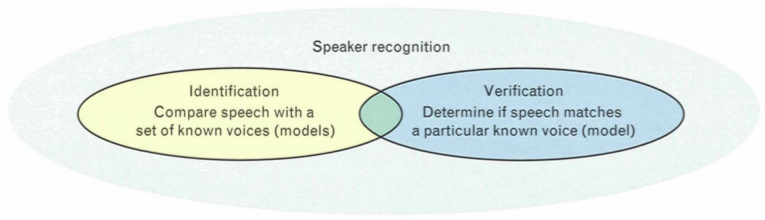
\includegraphics[width=\textwidth]{chapters/introduction/speaker-recognition}
    \caption{Relation between identification and verification of speakers, \refbib{Reynolds}{reynolds.1995a}.}
    \label{fig:speaker-recognition}
\end{figure}

The text inputted may be constrained, such as by type (e.g., digits and letters) or by number of words used (e.g., one word or sentences). In \textbf{text-dependent} systems the speech content is relevant to the evaluation, and the testing texts must belong to the training set, \refbib{Hébert}{hebert.2008}. A change in the training inputs demands a completely new training session. \textbf{Text-independent} systems have no input restrictions in both sets, with the non-textual characteristics of the speaker's voice (e.g., pitch and accent) being the important aspects to the evaluator. These characteristics are present in different sentences, use of foreign languages and even gibberish. Between the extremes falls the \textbf{vocabulary-dependent system}, which restricts the speech to come from a limited vocabulary (e.g., digits, such as ``two" or ``one-two-three"), \refbib{Reynolds}{reynolds.1995a}.

\section{Gaussian Mixture Models}
\label{sec:gmm}

This project is focused on \textbf{text-independent speaker recognition}, and as independence of the spoken message is a key characteristic of the problem, the most appropriate approach is to consider the training data as a stochastic variable. The most suitable distribution to represent random data is the Gaussian (or normal), leading to the choice of Gaussian Mixture Models (GMMs) to model the ASR systems.

Recognition systems are constructed using several techniques based on GMM. For identification, a GMM is trained for each enrolled speaker, referred to as Single Speaker Gaussian Mixture Model (SSGMM), with the identity given by the model with higher probability. Conversely, verification systems are designed using an Universal Background Model (UBM) trained to represent all speakers as a single background and a SSGMM or a Bayesian adaptation of the UBM, \refbib{Brown, Lee and Spohrer}{brown.lee.spohrer.1983}, named Single Speaker Adapted Gaussian Mixture Model (SSAGMM) to represent each speaker. A likelihood ratio test is used to evaluate a speech signal and to decide if it belongs or not to the identity claimed by the tested speaker.

Besides the previously cited, a new model using the theory of Fractional Covariance Matrix (FCM), \refbib{Gao, Zhou \& Pu}{gao.zhou.pu.2013}, named Fractional Gaussian Mixture Model (FGMM), is examined and compared with the traditional speaker identification, aimed to verify a possibility of improvement in the outcomes. All GMM designs are explained in details in \chapterref{gmm}, as well as their implementations and experiments in \chapterref{experiments}.

\section{Objectives}

This project implements ASR systems for the identification and verification processes and analyze the following:

\begin{itemize}\itemsep0pt
    \item Success rates for speaker identification with GMM and FGMM, using different sizes of mixture and features.
    \item Comparison between GMM and FGMM for speaker identification.
    \item False detection and false rejection rates for speaker verification with GMM and Adapted GMM (AGMM), using different sizes of mixture and features.
    \item Comparison between GMM and AGMM for speaker verification.
\end{itemize}

\section{Document Structure}

\chapterref{speaker-recognition-systems} contains basic information about ASR systems, as well as their basic architectures. The feature extraction process is explained in \chapterref{feature-extraction}, since the reasons for its use until the chosen technique (Mel-Frequency Cepstral Coefficient, MFCC). In \chapterref{gmm} the theories of GMM, UBM, AGMM and FGMM are presented. Experiments are described in \chapterref{experiments}, as well as their results. Finally, \chapterref{conclusion} concludes the study and proposes future works. Furthermore, \appendixref{results-identify-ssfgmm} presents tables and figures for speaker identification with FGMM, while \appendixref{results-verify} presents tables and figures for speaker verifications with GMM and AGMM.